\documentclass[../main.tex]{subfiles}

\begin{document}
\section{Discussion}
\label{sec:Discussion}
Thus far, we have found that the decline in the NRI has partly been caused by demographic factors and will have implications for policy choices. To pinpoint possible weaknesses related to this result, we discuss the assumptions we made when calibrating the model to nuance limitations and analytical suitability. Secondly, we discuss an extension of a more sophisticated financial sector that might capture some of the weaker points and discuss whether this extension will imply major consequences for essential dynamics in the model. Lastly, we discuss the role of openness. 

\subsection{Model selection}
\label{sec:Discussion.MS}
We have applied an OLG-model, a well-known procedure when investigating demographic tendencies and the role of pension systems. Obviously, there are several debateable simplifications that might not hold in reality. 

Our empirical measure of labour productivity $z_j$ is hourly labour income that includes wages and self-employment. The omission of a time subscript indicates that the relative productivity relationship between cohorts is constant over time. This might seem a controversial assumption. However, we are not aware of any literature which points to major changes in Danish relative wages between 1985-2020 that might alter our results. Combined with the fact that we want to keep the model tractable, we have limited reason to change the assumption of a constant relationship between age and productivity over time.

Another potential weakness of the model is that bequests are redistributed evenly to all agents in the economy in true altruistic fashion. It is more straightforward to have evenly distributed bequests for computational simplicity. Still, there might be a higher incentive to accumulate wealth if this wealth is kept within families. The absence of an intentional bequest motive is a standard debate in OLG literature. E.g. \textcite{gagnon2021understanding} discuss that this is likely to slightly weaken the size of the decline in the NRI due to intertemporal substitution between generations. The very nature of intentional bequests are clearly observed in today's society, but the effect on the NRI is unclear, and most cross-generation bequests often come in the form of housing which is beyond the scope of this thesis. 

In line with the above, it is also assumed that assets are zero when agents enter the model at the age of 20 and converge towards zero when agents reach 100. First, it is a well-known fact that not all young people are equal in wealth accumulation and inheritance. Secondly, we do not observe a strict convergence towards zero for retirees' assets in data. This might be because we do not account for housing in our model or intention to bequeath wealth for future generations. However, we clearly observe that assets (net wealth) on average are close to zero for agents at the age of 20 and declining for retirees. Thus, trends in data match the model characteristics. 

It is important to be aware of these simplifications, which possibly can be accounted for in a future specification. However, we would argue that these assumptions do not have any major impacts on the dynamics between demographics and the NRI while keeping the model tractable.

\subsection{Possible extension to the model}
\label{sec:Discussion.Pettm}
In the model, we abstract from uncertainty/risk, i.e. all assets are perfect substitutes and pay the same risk-free return. A recent paper by \textcite{marx2019return_on_capital} reflects on the notion that while risk-free interest rates have fallen, return on assets has not. This is mainly due to the perception of risk, according to the authors. They use a three-period OLG model with one source of risk. They instead allow for different asset classes - either agents own risky capital used in production or lend to the next generation. In this paper, we only account for contemporary cross-generation lending. Thus the authors can then differentiate between the evolution of interest rates and the risk premium associated with owning a more risky capital stock. To that end, we could extend the model to feature a more sophisticated financial sector where all assets are no longer perfect substitutes.

Most importantly, \textcite{marx2019return_on_capital} find that combined contribution of ageing and slowdown in productivity accounts for about 1 to 1.5 percentage points of the decline in risk-free interest rates in developed economies (Euro Area and the USA). Our findings for a similarly developed Danish economy are very much in line with these results based on a model with a more sophisticated financial sector. This suggests that despite the differentiation between asset classes, demographic factors remain important and have approximately the same impact on risk-free interest rates.

\subsection{The role of openness}
\label{sec:Role_of_openness}
As we model an open economy, we find it interesting to discuss the role of openness when determining the NRI. Recall that the risk parameter $\xi$, in essence, defines how open our model economy is. Hence, it captures how freely capital flows across borders and the behavioural features of investors, such as preferences for investing in domestic markets due to familiarity with the rules of the game. Consider the two extremes: For $\xi \rightarrow 0$, the model is completely open, and thus the Danish economy would fully import the world interest rate. In this case, no Danish process would affect the domestic NRI, as the development comes solely from abroad. For $\xi \rightarrow \infty$, the model becomes completely closed as the wedge/risk premium for any level of  trading foreign assets is too large for agents to consider trading. Thus, total capital in the economy effectively becomes domestic.

To illustrate the impact of openness, consider Figure \ref{fig:open_or_closed}. Despite a general major difference between modelling a closed or open economy, the effects on the NRI are minor. This is mainly due to similar demographic processes found in Denmark and the non-EA G7 countries and the assumption of a common TFP growth, both of which govern changes to the NRI. Even though a closed model implies a higher Danish natural interest rate in 1980s and 1990s by about 0.3-0.4 percentage points compared to that of the non-EA G7 countries (denoted world in the Figure \ref{fig:open_or_closed}), the differences even out following the secular decline in the 2000s. One may note that the decline is somewhat steeper in the 2000s than that of the world interest rate. This can be led back to low public debt levels in Denmark that reflect negatively on the NRI.

Thus to summarize, the openness of the economy does not seem to have a significant impact on the Danish NRI. 

\begin{figure}[H]
    \centering
    \caption{The role of openness}
    \label{fig:open_or_closed}
    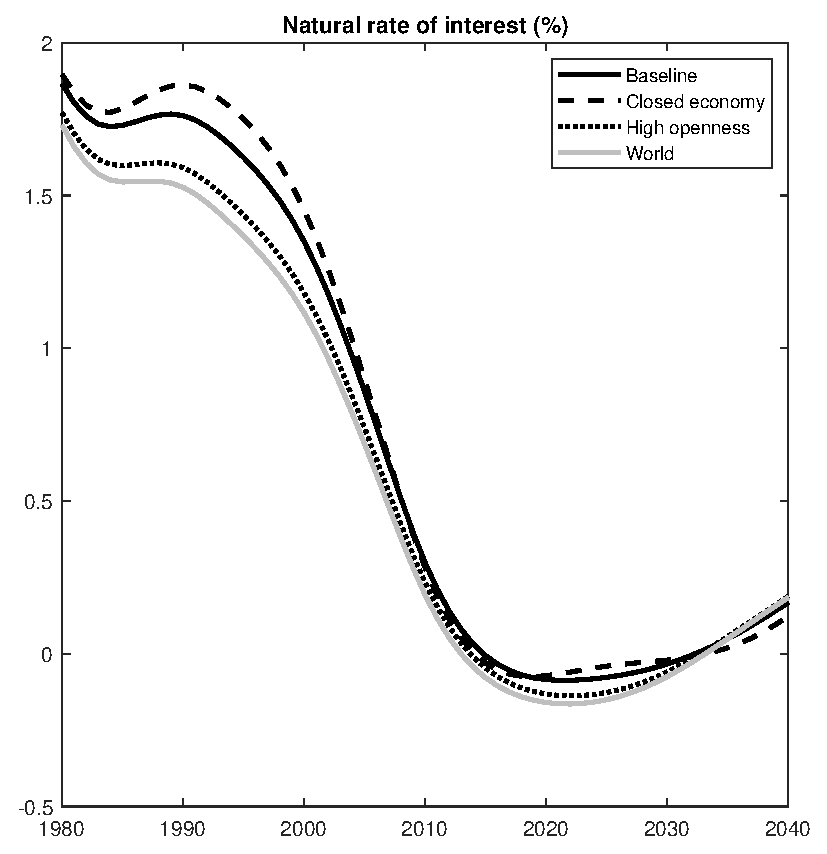
\includegraphics[]{Figures/Figure_9.eps}
    \begin{fignote}
    \end{fignote} 
\end{figure}


\end{document}